\documentclass[12pt ,a4paper ]{article}

\usepackage[utf8]{inputenc}
\usepackage[T1]{fontenc}      % caractères français
\usepackage[french]{babel}  %langue
\usepackage[left=2.3cm,right=2.5cm,bottom=2cm,top=2.3cm]{geometry}   % marges
\usepackage{verbatim}
\usepackage{float}
\usepackage{graphicx}         % images
\usepackage{verbatim}
\usepackage{multicol}
\usepackage{titlesec}

\usepackage[hyphens]{url}
\usepackage{hyperref}
\hypersetup{
    colorlinks=true,
    linkcolor=black,
    urlcolor=blue,
}

\urlstyle{same}


                           
\begin{document}
	\begin{titlepage}
		
		\vspace{0.5cm}
		\begin{center}		
			{\Large  Master 1 Informatique}
		\end{center}
		\vspace{1cm}
		
		\rule{1\linewidth}{1.1pt}\newline   %regle
		\begin{center}
			 {\Huge \textbf{Rapport de Projet : Neural Network And Learning}}
		\end{center}
		\rule{1\linewidth}{1.1pt} \\
		
		\begin{center}
		\begin{LARGE}
		\textbf{Sujet :} \\\vspace{0.6cm}  Construction d'un classificateur de photo de scènes naturelles
		\end{LARGE}
		\end{center}
		
		\vspace{0.5cm}
		\begin{center}	
				\begin{Large}
				Yann MARTIN D'ESCRIENNE \\ 
				Yohann TOGNETTI \\ 
				\end{Large}
		\end{center}
		\vspace{6cm}
		
		\begin{center}
			{\large « Année universitaire 2020 - 2021 »}
		\end{center}
		

\end{titlepage}

\newpage
\tableofcontents 
				
\newpage


\begin{multicols}{2} 
\section{Présentation générale du projet}
		Dans le cadre de notre cours de Neural Network and Learning, il nous a été demandé d'effectuer un projet impliquant une intelligence artificielle travaillant sur des images. Celle-ci a pour but de construire un classificateur de photo de scènes naturelles comme ceux qu’on pourrait intégrer dans un appareil photo intelligent qui à chaque prise de photo va taguer l’image avec le nom d’une catégorie qui y correspond. 
	
		
\section{Descriptif du sujet et ses finalités}
\subsection{Descriptif du sujet}
	Ainsi, pour entrer dans les détails le but qui est de "taguer l'image" correspond au fait de la catégoriser grâce à un classificateur entrainé possédant les catégories de scènes naturelles désirées. Pour cela avons dû utiliser un réseau neuronal convolutif étant donné que nous traitons des images. Une fois la réponse du classificateur reçue, elle correspond initialement à un entier, nous avions donc le devoir de le convertir en tag correspondant au nom de la catégorie trouvée. \\
	
	
	L'affichage du résultat doit se faire à l'aide d'une méthode \textit{predict} qui prend en entrée le chemin de fichier d’une image et une chaine de caractères 'mode' qui renvoie le nom de la catégorie correspondant à l'image si \textbf{mode='category'} où un vecteur de probabilités si \textbf{mode='probabilities'} ou chaque éléments du vecteur indique la probabilité que l'image appartienne à la catégorie correspondante.

\subsection{Les catégories}
Celles-ci sont au nombre de 6, chacune correspond à une catégorie de paysage ou de scène naturelle de la liste suivante : 

\bigskip
\begin{itemize}
\item buildings
\item forest
\item glacier
\item mountain
\item sea
\item street
\end{itemize}

\bigskip
\textit{Building} correspond ainsi à des bâtiments comme une maison ou un immeuble qui se trouve généralement dans une ville. \\
\textit{Forest} comme son nom l'indique correspond à un paysage forestier avec la présence ou non d'animaux. \\
\textit{Glacier} quant à lui représente une montagne enneigée ou bien un glacier ou morceaux de glace de la banquise, cette catégorie est extrêmement corrélée avec \textit{Moutain} car celle-ci correspond à une montagne pouvant parfois aussi être enneigé. Le découpage n'est pas toujours pertinent et encore plus ici, nous en parleront dans la section \textit{Description des données}.\\
 \textit{Sea} représente les décors marins en général, que ce soit une plage, la mer avec ou sans terre ferme, ou bien même un décor sous-marin, tout cela va dans cette catégorie. \\
Enfin la catégorie \textit{Street} met en avant une rue, qui peut donc facilement se rapprocher de \textit{building} étant donnée la présence quasi-permanente de bâtiments dans une rue, on y trouve souvent des passant et des voitures.  

\newpage
\section{Description des données}

\subsection{Le jeu de données}

	Les données utiliser pour pouvoir réaliser cet apprentissage viennent du jeu de données « Intel Image Classification ». Ce jeu de données est composé d’un totale de 24.347 images et elles sont toutes de taille 150x150 px. Le jeu de données est réparti en trois fichier, seg\_train, seg\_test et seg\_pred. \\
Pour les fichiers de train et de test, sont tous deux repartis en 6 sous fichier qui sont nos classification (street, buildings, …) et qui possèdent chacun les image classifier correspondantes.\\
Le fichier train possèdent en tout 14.046 image repartie avec les proportions plutôt équivalente comme nous pouvons le voir :

\begin{itemize}
\item Buildings 2.191 images
\item Forest 2.271 images
\item Glacier 2.416 images
\item Mountain 2.512 images
\item Sea 2.274 images
\item Street 2.382 images
\end{itemize}

Le fichier test possèdent en tout 3000 image repartie avec les proportions plutôt équivalente comme nous pouvons le voir :

\begin{itemize}
\item Buildings 437 images
\item Forest 474 images
\item Glacier 553 images
\item Mountain 525 images
\item Sea 510 images
\item Street 501 images
\end{itemize}
Les deux jeux de données ont un nombre de données plutôt important pour chaque classe, cela est plutôt favorable pour pouvoir faire une classification correcte.\\
Le dernier répertoire, celui de tes possèdent 7.301 qui sont de toutes classe.

\subsection{Des données pas forcement bien classifiée}
L’une de nos découvertes sur les jeux de données était que certaine image était mal classifiée. Voici certains exemples qui illustre nos propos :

\begin{figure}[H]
\begin{center}
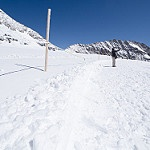
\includegraphics[scale=1]{./img/20662.jpg}
\caption{\small{Image 20662.jpg, catégorie Mountain du jeu de test.}}
\end{center}
\end{figure}
 
\begin{figure}[H]
\begin{center}
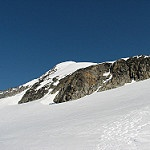
\includegraphics[scale=1]{./img/23589.jpg}
\caption{\small{Image 23589.jpg, catégorie Glacier du jeu de test.}}
\end{center}
\end{figure}
Ces deux images n’ont pas la même catégorie et pourtant, elles se ressemble fortement car ce sont de montagne enneiger. Les catégorie Mountain et Glacier sont toutes deux correct, mais dans ce cas-là l’ia vas surement se tromper sur l’une des deux.\\
Un autre type de problème sont les images hors contexte donc difficilement classifiable comme celle-là :
 
\begin{figure}[H]
\begin{center}
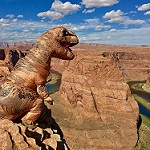
\includegraphics[scale=1]{./img/1512.jpg}
\caption{\small{Image 1512.jpg, catégorie glacier du jeu de train.}}
\end{center}
\end{figure}
Certaines images vont donc automatiquement faire descendre la précision car même pour un nous il est difficile de classifier comme ce qui est attendue. Néanmoins, La plupart des autres données sont correct et vont nous permettre de faire une bonne classification.

\newpage
\section{Implémentation de l'algorithme}
Notre algorithme est développé en python. Il se trouve dans le fichier \textit{Program.py} et possède 3 méthodes majeures qui ont permis de répondre aux attentes du sujet. Nous allons donc présenter chacune de ces méthodes avec un peu plus de détails. \\

La réussite de ce sujet est grandement due au livre \textbf{L'APPRENTISSAGE PROFOND AVEC PYTHON} de \textit{François CHOLLET}. La lecture de son travail nous à permis un apprentissage rapide du fonctionnement des réseaux neuronal convolutif ainsi que leur mise en application pour notre IA. 

\subsection{preprocessing}
Cette méthode prend comme argument le directory qui contient les images avec la structure décrite dans la partie \textit{Description des données} afin d'effectuer le pré-traitement. \\

Dans un premier temps cette méthode va donc créer un répertoire pour les données d'entrainement, puis un autre pour les données de validation en ce basant sur le répertoire donné en argument.\\

Ensuite, deux \textit{ImageDataGenerator} vont être créer avec une mise à l'échelle de 1/255. En effet il est beaucoup plus simple pour l'IA de travailler avec des données entre 0 et 1 que 0 et 255 concernant le RGB de chaque pixels. Le premier ImageDataGenerator va servir pour les données d'entrainement et le deuxième pour la validation.\\

Finalement deux générateurs vont être créés pour les deux parties avec comme taille voulue 150x150 pixels étant donnée que cela correspond à la taille des images dans le jeu de données. Le \textit{batch\_size} est de \textbf{32} et le \textit{class\_mode} est en \textbf{binary} étant donné que nous avons comme résultat un vecteur constitué de 0 et de 1.\\

Les générateurs d'entrainement et validation ainsi créés vont être retourné par la méthodes afin de les utiliser dans les autres. 

\subsection{trainModel}
Cette méthode à pour but de créer et entrainer le modèle. Elle prend en argument les deux générateurs créés à la partie précédente, ainsi que des paramètres propres à l’entrainement de l’ia comme le nombre d’epoch, le nombre d’étape par epoch ainsi que le chemin d’enregistrement du modèle qui sera créé.\\

\subsubsection{Description du modèle}
La construction de notre modèle actuel est comme ci-dessous : 

\begin{figure}[H]
    \begin{center}
        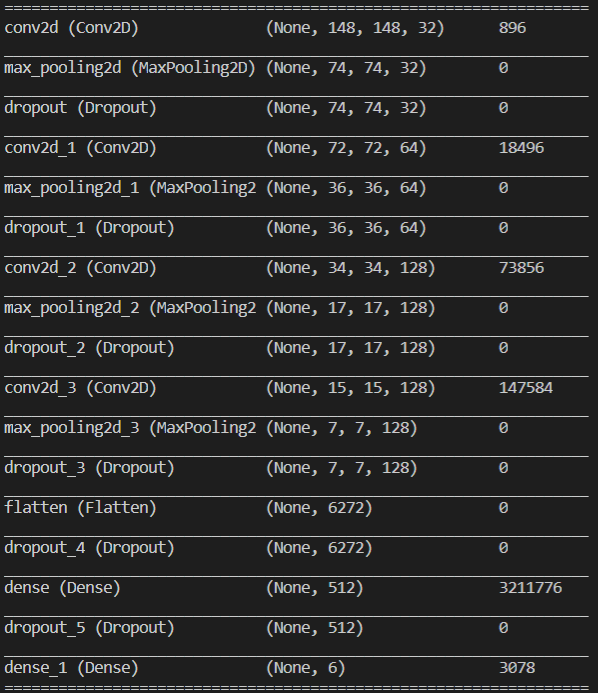
\includegraphics[scale=0.62]{./img/model_sum.png}
    \end{center}
\caption{\small{Résumé du model}}
\end{figure}

La partie principale de notre modèle se constitue donc de plusieurs blocs composés de la manière suivante : un \textbf{2D convolution layer}  suivi d'un \textbf{Max pooling operation for 2D spatial data} et se terminant par un \textbf{dropout layer}. A la fin de ces paternes un \textbf{flatten layer} est mit en place suivi d'un nouveau \textbf{dropout}. Notre modèle se termine enfin par deux \textbf{dense layer} avec un autre \textbf{dropout} entre eux \\ 

Les convolution layers utilisent tous de strides de taille 3x3 et ont pour fonction d'activation \textit{Rectified Linear Unit}. Le première couche utilise comme input\_shape des images RGB de taille 150x150 afin de s'adapter à nos données.\\
Les maxpooling layers ont quant à eux un strides de taille 2x2.\\
Tout les dropout mis en place dans ce modèle ont comme paramètre 20\% des données abandonnées. Ceci afin de limité l'overfitting de nos données. \\
Le premier dense layer prend comme paramètre 512 dimensions avec comme fonction d'activation \textit{Rectified Linear Unit} et utilise également un \textit{kernel\_regularizer}. Le deuxième quant à lui possède 6 dimensions, étant donné que l'on souhaite 6 classes et utilise \textit{softmax} comme fonction d'activation. \\

La compilation du modèle se fait avec un optimiser \textit{adam} et une fonction de perte \textit{categorical\_crossentropy} et se focalise sur la précision du modèle. \\

Finalement nous entrainons le modèle avec les paramètres donnés précédemment et le stockons dans history afin d'afficher sur un graphe l'évolution de la précision au cours de l'entrainement. Nous sauvegardons au passage le modèle dans le chemin donné en argument. 

\subsubsection{Evolution du modèle}
Grâce au nombreux exemples du livre qui nous à servis de base, notre premier modèle possédait déjà une précision aux alentours de 80\% pour les données de validation et 98\% pour celle d'entrainement. Ceci était déjà un très bon résultat mais notre modèle souffrait donc d'\textbf{overfitting}.\\

Nous avons remédier au problèmes en utilisant des dropout layers afin que notre modèle ne se focalise pas trop sur ses données d'entrainement uniquement. Nous avons choisi d'abandonner 20\% de nos résultat après chaque paternes conv2D/maxpooling. On peut ainsi constater la différents de précisions des données de validation dans les graphiques suivant : 

\begin{figure}[H]
    \begin{center}
        \includegraphics[scale=0.4]{./img/figure_3.png}
    \end{center}
\caption{\small{Précision sans dropout}}
\end{figure}

\begin{figure}[H]
    \begin{center}
        \includegraphics[scale=0.4]{./img/figure_1.png}
    \end{center}
\caption{\small{Précision avec dropout}}
\end{figure}

On voit alors très clairement que la précision de validation est beaucoup plus proche de celle d'entrainement même si celle-ci à donc tendance à être plus basse, s'expliquant par l'abandon de 20\% des résultats obtenus. 

\subsection{predict et méthodes graphiques}
Cette méthode correspond aux attentes du sujet pour afficher les prédictions de notre modèle avec le mode attendu qu'il prend donc en argument. Il prend également pour paramètre le modèle entrainé ainsi que le chemin de fichier de l'image à prédire. 

Enfin, pour mettre sous forme de diagramme ou de graphiques les résultats obtenus qui seront présentés dans la section suivante, nous nous sommes appuyer sur la librairie matplotlib. Nous avons donc mit en place différentes méthode pour ceci, ainsi qu'un autre programme appelé \textit{report.py} pour l'affichage graphique de la matrice de confusion. 

\subsection{Temps d'apprentissage du modèle}
Le temps d'apprentissage du modèle dépend bien évidemment du nombre d'epoch ainsi que du nombre d'étapes par epoch choisi. Notre modèle final se base sur 60 epoch de 430 étapes chacune. Bien évidemment lors de nos test d'améliorations, nous ne mettions que 30 epoch de 120 étapes afin de voir rapidement les résultats. \\

Sur le pc le plus performant du groupe, le modèle final prend environ 15-20 min pour s'entrainer et lors de nos test environ 2-3 minutes. Cela viens du fait de l'utilisation de l'installation des dll utilisant la carte graphique et cœurs cuda pour l'apprentissage de l'IA. Néanmoins ce temps dépend bien sur fortement du matériel utilisé et de sa configuration.  


\newpage
\section{Résultat obtenus}
Il est à noter que les résultats peuvent être légèrement différent à chaque entrainement du programme ainsi les graphiques qui vont suivre ne sont pas forcément absolus. 

\subsection{Résultat général}
Pour commencer, je vais présenter nos résultats de manière général. Au niveau de la « precision », le « recall » et « f1-score », nous avont une moyenne de 88\% ce qui est un score plutôt satisfaisant.\\
Maintenant, nous allons légèrement décomposer ce score, voici un graphique reprenant les différentes catégories.\\
Ce graphique nous permet pour chaque classe de voir comment l’IA a réussi à classifier pour chacune de classe. Pour chaque classe nous avons 3 données, le recall, la precision et le f1-score.\\
Le f1-score est un mixte des deux et est donc l’élément le plus favorable à regarder.
Tout d’abord, nous pouvons voir que la classe « forest » est la plus facile à repérer pour l’IA avec un f1-score de 96\% ce qui est plus qu’acceptable. De plus, il arrive rarement que l’on assigne cette classe a une image qui n’est pas une forêt (« recall » a 99\%).
De plus, la classe « mountain » est la classe qui a le moins bon f1-score mais qui reste plus qu’acceptable étant donné qu’il est a 83\%. \\
\end{multicols}

\begin{figure*}[h]
    \begin{center}
        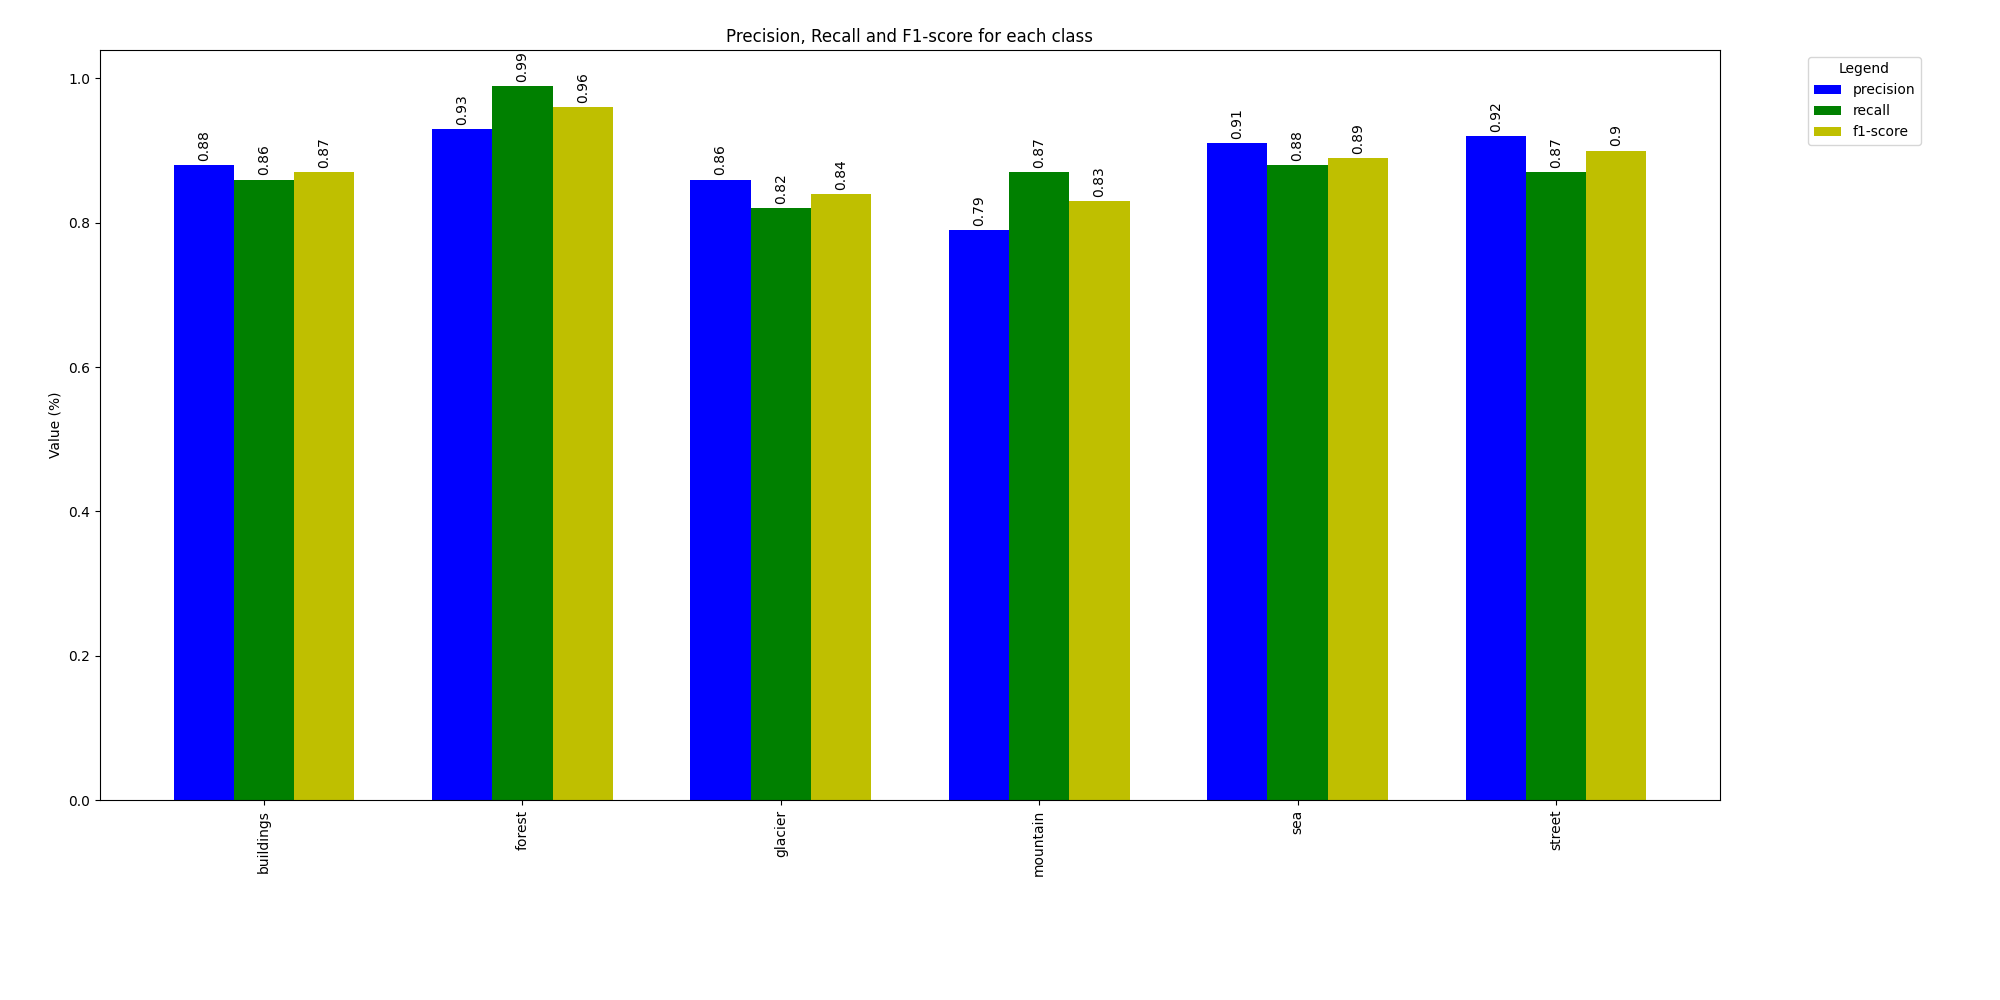
\includegraphics[width=1.15\textwidth]{./img/class_plot.png}
    \end{center}
    \caption{Statistique général de chaque classe}
\end{figure*}
\begin{multicols}{2} 

\subsection{Analyse des classes détailler}

Maintenant, nous allons voir plus précisément les erreurs de notre IA. Pour cela nous allons utiliser le graphique suivant montrant le recall pour chaque catégorie.\\
Si nous regardons la classe buildings, nous pouvons voir que le recall vient principalement de la classe Street avec 8.01\% des élément qui on était classé en buildings alors qu’il devait être classifier en street. Nous retrouvons aussi l’inverse avec 8.18\% en street alors qu’il devait être en buildings. Cela peut s’expliquer facilement, tout d’abord, les deux classes représente généralement des villes, sur une même photo, il peut y avoir une rue et un bâtiment. Dans ce cas-là il peut être difficile à l’IA de pouvoir dire si la photo veut montrer principalement une rue ou les bâtiments qui l’entoure.\\
La deuxième comparaison que nous pouvons faire est celle entre « glacier » et « mountain ». Pour ces deux classes, il y a un pourcentage de classification en montagne de 13.02\% alors que ce sont des glaciers et de 9.33\% pour l’inverse. Cela est du a notre jeu de données. Comme bue précédemment (cf. 3.2), il y a beaucoup d’image sans glace qui sont considérer comme des glaciers et d’image de montagne geler qui peuvent être trouver dans le jeu de données de ces deux catégories.\\
En ce qui concerne la classification « sea », nous pouvons voir que l’on a certaine photo ou l’on voit de l’eau comme des lac, la mer ou encore des rivières. Il est probable que la probabilité de 6\% soit du a ce type d’image mais il doit être possible d’améliorer celle-ci.\\
Pour finir, la classe « forest » qui avait des résultats vraiment satisfaisant, nous pouvons le constater aussi sur ce graphique avec très peut de présence des autre classe.\\

\end{multicols}
\begin{figure*}[h]
    \begin{center}
        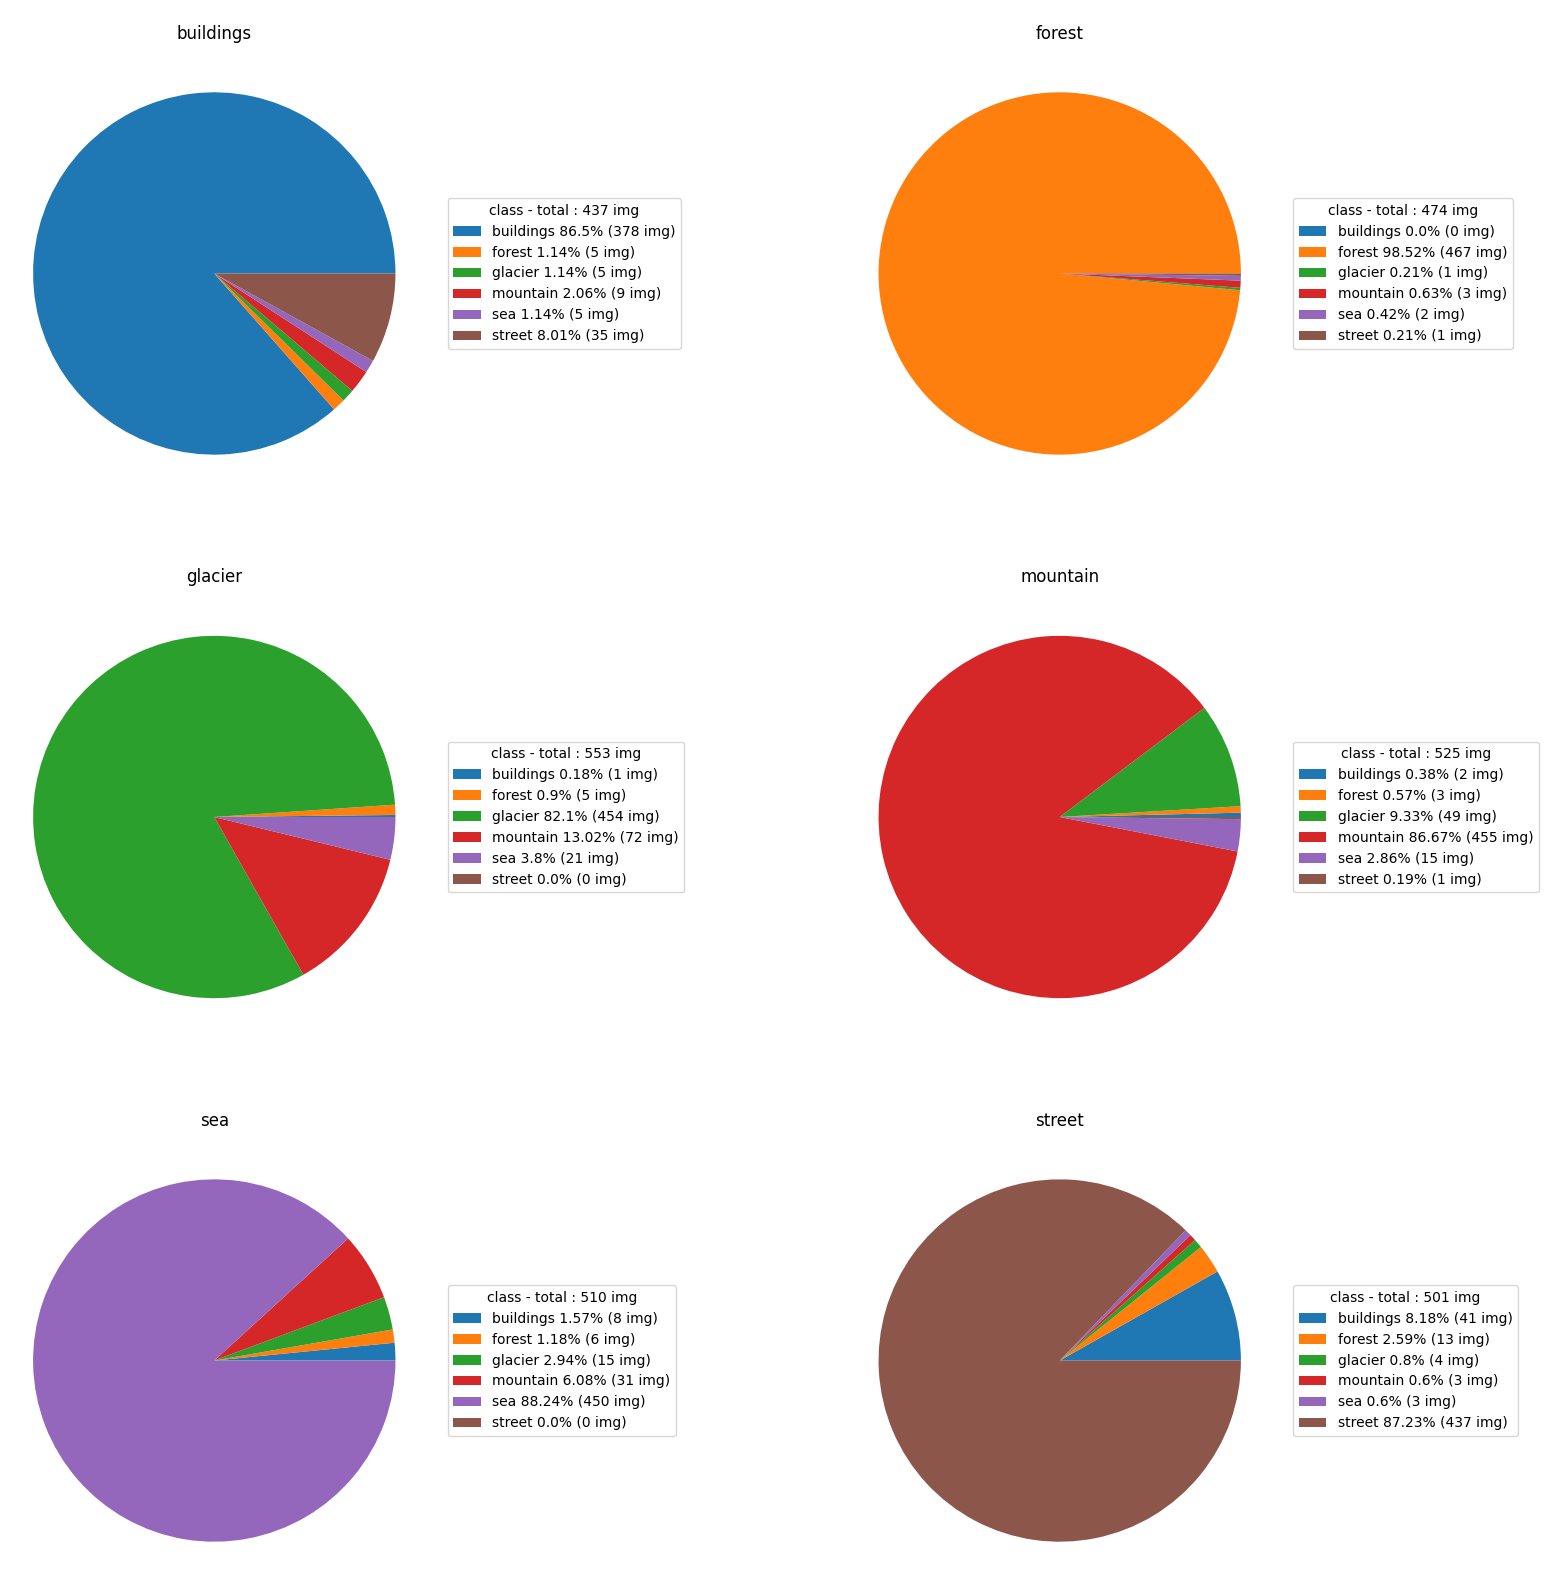
\includegraphics[width=0.95\textwidth]{./img/pie_diagram.png}
    \end{center}
    \caption{Recall de chaque classe}
\end{figure*}

\newpage
\begin{multicols}{2} 

\newpage
\section{Les améliorations possibles}
Globalement, pour nous ce projet n'a pas tant d'amélioration à faire que cela. Les nombres de données pour construire le modèle est largement suffisant, il n'y a donc pas eu à recourir à des transformations d'image pour lutter contre un manque de données. Elles sont plutôt diverses et équilibrées, il ne faut donc pas mettre en place de système de pondération pour les classes.\\

\subsection{Travail sur le jeu de données}
Comme expliqué précédemment, le jeu de données met certaines images dans des classes qui n'ont pas toujours un réel rapport ou alors en met d'autres quasiment identiques dans des classes différentes. Résoudre ce problème en supprimant ou déplaçant toutes ces images problématiques dans les bonnes catégories permettrait alors à l'IA de mieux savoir différents ces différentes images et ainsi obtenir une meilleure précision. 

\subsection{Travail sur le modèle}
Bien évidemment, notre modèle est loin d'être parfait. Par manque de temps, nous n'avons pas expérimenter toutes les possibilités et d'autre méthodes d'apprentissage de classifications d'image existent. Notre précision (~87\%)  reste néanmoins plus que correcte, mais il aurait peut être été possible d'atteindre 90\%. 

\end{multicols}
\newpage
\section{Conclusion}
Pour conclure sur notre travail sur le sujet donné, l'apprentissage et la construction du modèle de fût pas le plus difficile à mettre en place et obtenir rapidement une bonne précision. \\
Cela s'explique par le très bon livre donné en référence de François CHOLLET, celui-ci contenait toutes les informations nécessaire à la réussite du sujet mais aussi à l'apprentissage profond neuronal en général.  Certaines solutions pour lutter contre l'overfitting y était même présente. Il nous a ainsi fallu compléter toutes ces informations par quelques recherches supplémentaire sur internet afin d'obtenir notre résultat final.\\
La classification d'image étant quelques choses que nous n'avions encore jamais abordé, nous avons donc pu constater que ce n'est pas excessivement compliqué. A présent, nous avons le savoir minimal nécessaire afin d'étendre la classification d'image à n'importe quels problèmes pouvant être assimilé à ce projet, la seule différences étant le jeu de données et les catégories différentes. 

\section{Membres du groupe}
\subsection{Yann MARTIN D'ESCRIENNE}
Ce projet m'a beaucoup apporté. Il est pour moi une bonne finalisation de tout les TPs que nous avons pu faire en Neural Network and Learning. Le confort du bon jeu de données m'a permis de mieux m'investir dans le projet, malgré quelques surprises dans certaines catégories.\\

Nous avons travaillé en groupe quant à l'implémentation du modèle mais également dans tout le projet en général, avançant ensemble de façon synchrone sur le projet. J'ai majoritairement travaillé sur la phase de preprocessing et de prédiction. J'ai également recherché de nombreuses informations dans le livre de François CHOLLET afin de pouvoir répondre à toutes nos questions et attentes du sujet. 
Je me suis occupé de rédiger les parties 1,2,4,6 et 7 du rapport. 

\subsection{Yohann TOGNETTI}

\section{Références}
\begin{itemize}
\item Deep Learning with Python by François Chollet 
\item TensorFlow Conv2D Layers: A Practical Guide :\\ \url{https://missinglink.ai/guides/tensorflow/tensorflow-conv2d-layers-practical-guide/}%
\item Keras documentation :\\ \url{https://keras.io/api/layers/}%
\item Overfit and underfit  |  TensorFlow Core :\\ \url{https://www.tensorflow.org/tutorials/keras/overfit_and_underfit#strategies_to_prevent_overfitting}%
\item Image classification  |  TensorFlow Core :\\ \url{https://www.tensorflow.org/tutorials/images/classification}%
\item WIKIPEDIA FR :\\ \url{https://fr.wikipedia.org/wiki/Wikip%C3%A9dia:Accueil_principal}%
\end{itemize}




\end{document}